\section{Background and Motivation}
% 背景与动机
\label{sec:background}
\subsection{GPU Systems and Workload Diversity}
% GPU 系统与负载多样性
\label{sec:arch-gpu}

% \arq{I think this is too many ideas for one paragraph  It should probably reference Figure 1 (!)}
As shown in \Cref{fig:motivation_silos}, we focus on three GPU resource management domains across the software stack: memory placement and migration, compute scheduling, and on-device thread scheduling.
% 如 \Cref{fig:motivation_silos} 所示，我们关注软件栈中三个 GPU 资源管理领域：内存放置与迁移、计算调度与设备端线程调度。
User-space frameworks (e.g., vLLM~\cite{kwon2023efficient}, Salus~\cite{yu2020fine}, PILOT~\cite{ravi2021pilot}) leverage application semantics (e.g., neural structures, latency constraints) to implement request scheduling and KV-cache offloading policies.
% 用户态框架（如 vLLM、Salus、PILOT）利用应用语义（如神经网络结构、延迟约束）实现请求调度与 KV 缓存卸载策略。
Kernel drivers manage memory, scheduling, and multi-tenant isolation via privileged hardware mechanisms (MMU, interrupts), typically using fixed, application-agnostic algorithms (e.g., LRU eviction) under Unified Virtual Memory (UVM), which transparently handles oversubscription through host-device page migrations.
% 内核驱动通过特权硬件机制（MMU、中断）管理内存、调度与多租户隔离，通常在统一虚拟内存（UVM）下使用固定的、与应用无关的算法（如 LRU 淘汰），UVM 通过主机—设备页迁移透明处理内存超配。
GPU devices execute kernels via SIMT (Single Instruction, Multiple Threads); on NVIDIA hardware, 32-thread warps run instructions in lockstep on SMs, with internal states (e.g., warp access patterns) opaque to host drivers.
% GPU 设备以 SIMT（单指令多线程）方式执行内核；在 NVIDIA 硬件上，32 线程的 warp 在 SM 上锁步执行指令，其内部状态（如 warp 访存模式）对主机驱动不可见。


\begin{figure}[t]
    \centering
    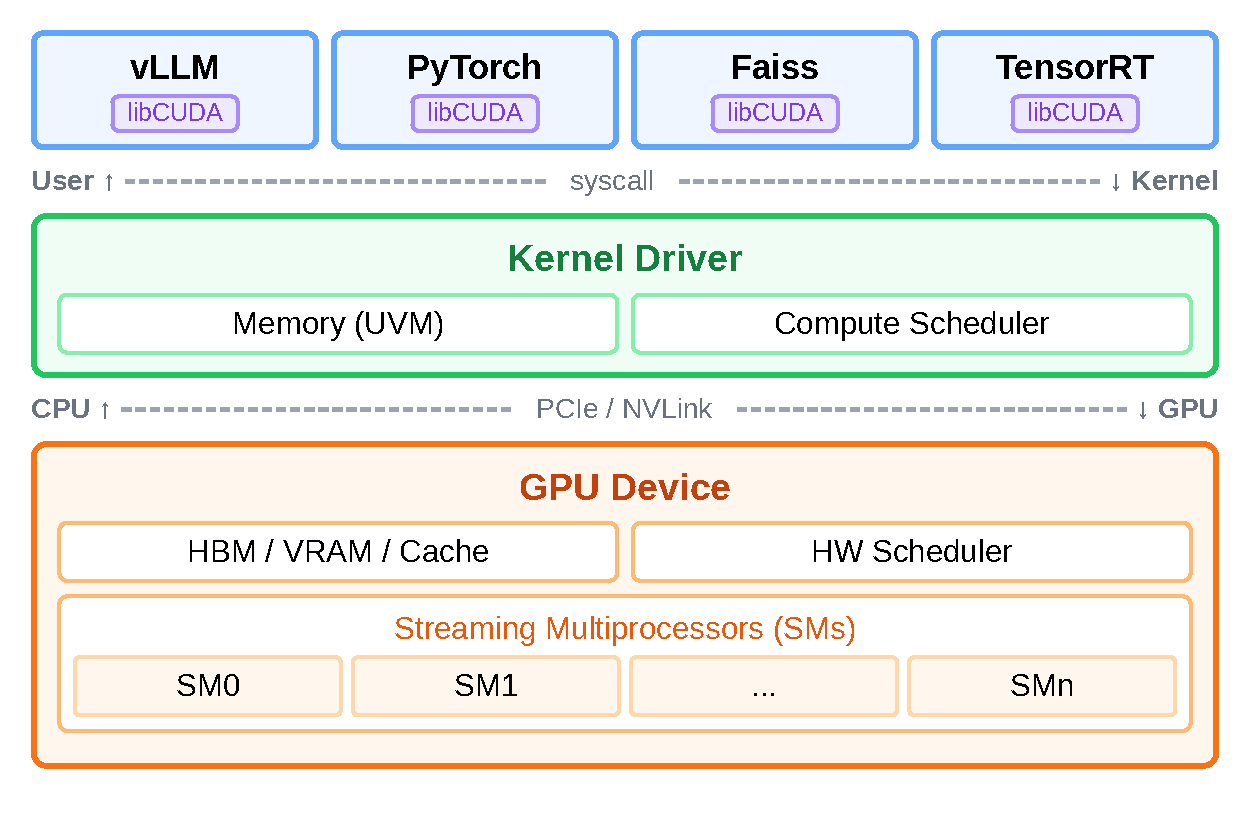
\includegraphics[width=\columnwidth]{img/gpu_stack_figure.pdf}
    \caption{GPU system stack: user-space frameworks, kernel driver (memory and scheduling), and GPU hardware.}
    % GPU 系统栈：用户态框架、内核驱动（内存与调度）与 GPU 硬件。
    \label{fig:motivation_silos}
\end{figure}

% \arq{I think this should be two paragraphs: one that talks about workload diversity and the second that then talks about the need for different policies.}
GPU workloads exhibit diverse resource access patterns.
% GPU 负载呈现出多样的资源访问模式。
Results from \sys{}'s eBPF-based tracing tools (\S\ref{sec:eval}) confirm this diversity: \Cref{fig:access_patterns} captures memory page-fault addresses over time under UVM, showing that LLM MoE inference exhibits periodic stride bursts from expert activations; GNN training shows irregular random access from pointer-chasing graph traversal; and vector search alternates between sequential scans (index build) and random probes (query)~\cite{pan2024survey,cao2023gpu}.
% \sys{} 基于 eBPF 的追踪工具（\S\ref{sec:eval}）的结果证实了这种多样性：\Cref{fig:access_patterns} 捕获了 UVM 下随时间变化的内存缺页地址，显示 LLM MoE 推理因专家激活呈现周期性步长突发；GNN 训练因指针跳转的图遍历呈现不规则随机访问；向量搜索则在顺序扫描（索引构建）与随机探测（查询）之间交替。
\Cref{fig:thread_scheduling} reveals a 127$\times$ SM scheduling load imbalance in a vector-add GPU kernel, invisible to host-side drivers.
% \Cref{fig:thread_scheduling} 揭示了向量加法 GPU 内核中 127$\times$ 的 SM 调度负载不均，主机侧驱动无法察觉。

These diverse patterns require workload-specific policies across all three domains.
% 这些多样的模式要求三个领域均采用面向负载的策略。
UVM eviction and prefetch policies alone can impact execution time by up to 73\%~\cite{ganguly2019interplay,park2025helm}: MoE inference favors specialized eviction over default LRU~\cite{sheng2023flexgen,kwon2023efficient}, while GNN training demands aggressive sequential prefetch~\cite{lin2024towards,wang2016gunrock}, but each can degrade other workloads.
% 仅 UVM 淘汰与预取策略就可使执行时间变化高达 73\%：MoE 推理偏好专用淘汰而非默认 LRU，而 GNN 训练需要激进的顺序预取，但两者都会损害其他负载。
Compute scheduling requires adaptive priority and preemption policies as multi-tenant demands fluctuate~\cite{fan2025gpreempt,wang2024gcaps}, and SM load imbalance benefits from custom thread scheduling.
% 多租户需求波动时，计算调度需要自适应的优先级与抢占策略，SM 负载不均则受益于自定义线程调度。
Yet current drivers and firmware enforce a single fixed policy.
% 然而现有驱动与固件仅强制执行单一固定策略。
\begin{figure*}[t]
    \centering
    
\includegraphics[width=\textwidth]{img/pattern/combined_patterns_1x5_v2.pdf}
    \caption{Page-fault address traces over time across four workloads. Each pattern implies a different optimal prefetch/eviction strategy; no single policy fits all.}
    % 四个负载随时间变化的缺页地址轨迹。每种模式对应不同的最优预取/淘汰策略；没有单一策略能适配所有负载。
    \label{fig:access_patterns}
\end{figure*}


\begin{figure}[t]
    \centering
    
\includegraphics[width=\columnwidth]{img/pattern/vector_add/thread_scheduling_motivation.pdf}
    \caption{GPU thread scheduling imbalance observed via eBPF tracing. (a) SM load distribution: 127$\times$ imbalance. (b) Warp activity heatmap across SMs.}
    % 通过 eBPF 追踪观察到的 GPU 线程调度不均。(a) SM 负载分布：127$\times$ 不均。(b) 跨 SM 的 warp 活跃度热力图。
    \label{fig:thread_scheduling}
\end{figure}

\subsection{Agent-Based Policy Exploration}
% 基于智能体的策略探索
\label{sec:motivation-agent}

Agentic OS policy exploration fits the large GPU policy space but requires programmable interfaces missing in current GPU stacks.
% 智能体化的 OS 策略探索契合庞大的 GPU 策略空间，但当前 GPU 软件栈缺少所需的可编程接口。
Unlike parameter-tuning methods, AI agents~\cite{dwivedula2025policysmith,zheng2025schedcp} directly generate and iteratively refine policy logic to explore richer, workload-specific strategies.
% 与参数调优方法不同，AI 智能体直接生成并迭代优化策略逻辑，以探索更丰富的面向负载的策略。
However, existing GPU stacks provide only fixed knobs (e.g., \texttt{cudaMemAdvise}, driver module parameters), lacking programmability needed for complex heuristics such as workload-aware eviction or adaptive prefetching.
% 然而现有 GPU 软件栈仅提供固定旋钮（如 \texttt{cudaMemAdvise}、驱动模块参数），缺少实现负载感知淘汰或自适应预取等复杂启发式所需的可编程性。

Effective GPU policy optimization requires an OS interface with three key properties: (1) \emph{safe}, robustly handling generated policies without kernel panics or GPU corruption; (2) \emph{dynamic}, rapidly deploying and iterating policies at runtime without application restarts or kernel rebuilds; and (3) \emph{full-stack}, observing GPU-internal states, coordinating across tenants, and controlling driver-level decisions like eviction and fault-path prefetching.
% 有效的 GPU 策略优化需要具备三个关键属性的 OS 接口：(1) \emph{安全}，稳健处理生成的策略，不引发内核 panic 或 GPU 损坏；(2) \emph{动态}，在运行时快速部署和迭代策略，无需重启应用或重新编译内核；(3) \emph{全栈}，可观察 GPU 内部状态、跨租户协调，并控制驱动层决策（如淘汰与缺页路径预取）。

\subsection{Limitations of Existing Approaches}
% 现有方法的局限
\label{sec:motivation-limitations}

% \arq{Make sure to critique these existing approaches by saying they are not safe, dynamic, or full-stack.}
Existing approaches fail to simultaneously provide a safe, dynamic, and full-stack programmable OS interface for GPU resource management.
% 现有方法无法同时提供安全、动态且全栈的可编程 OS 接口用于 GPU 资源管理。

\paragraph{Driver-Level Policies.}
% 驱动层策略。
Driver-level approaches either expose fixed knobs (e.g., \texttt{cudaMemAdvise}, driver module parameters) that select among preset behaviors, or embed custom logic directly into driver code.
% 驱动层方法要么暴露固定旋钮（如 \texttt{cudaMemAdvise}、驱动模块参数）在预设行为间选择，要么将自定义逻辑直接嵌入驱动代码。
Systems like TimeGraph~\cite{kato2011timegraph}, Gdev~\cite{kato2012gdev}, and OS kernel interception methods~\cite{kernelintercept} embed scheduling and memory-management logic into driver modules.
% TimeGraph、Gdev 等系统以及 OS 内核拦截方法将调度与内存管理逻辑嵌入驱动模块。
More recent work such as GPREEMPT~\cite{fan2025gpreempt} and GCAPS~\cite{wang2024gcaps} add priority-based preemption, and LithOS~\cite{coppock2025lithos} re-implements runtime stacks with OS-like abstractions.
% 更新的工作如 GPREEMPT 和 GCAPS 增加了基于优先级的抢占，LithOS 则以类 OS 抽象重新实现运行时栈。
Despite improved performance, all these approaches require OS kernel or driver modifications to change policy: they are neither safe (bugs can crash the OS kernel) nor dynamic (policy changes require recompilation and restarts), and still lack GPU-internal observability for full-stack control.
% 尽管性能有所提升，所有这些方法要改变策略都需修改 OS 内核或驱动：既不安全（bug 可崩溃 OS 内核）也不动态（策略变更需重编译与重启），且仍缺乏全栈控制所需的 GPU 内部可观测性。

\paragraph{Host User-Space Runtimes and Libraries.}
% 主机用户态运行时与库。
User-space frameworks~\cite{ng2023paella,gim2025pie,shen2025xsched,chen2025ktransformers,coppock2025lithos} offer programmability but face three limitations.
% 用户态框架提供了可编程性，但面临三大局限。
First, policies are application-bound, requiring per-framework implementation and preventing reuse across ecosystems.
% 第一，策略绑定于特定应用，需逐框架实现，无法跨生态复用。
Second, process-level isolation prevents cross-tenant visibility and coordinated memory-scheduling decisions across tenants~\cite{xiao2018gandiva,yu2020fine}; hardware partitioning such as MIG imposes fixed resource boundaries that cannot be dynamically rebalanced.
% 第二，进程级隔离阻碍了跨租户可见性与跨租户的协同内存—调度决策；MIG 等硬件分区施加了固定资源边界，无法动态再平衡。
Third, user-space code cannot access privileged driver mechanisms, leaving policies constrained to GPU kernel launch boundaries and unable to execute on latency-critical paths (e.g., page-fault handlers), perform precise preemption, or exploit GPU-side warp-level access patterns.
% 第三，用户态代码无法访问特权驱动机制，策略被限制在 GPU 内核启动边界，无法在延迟敏感路径（如缺页处理程序）上执行，无法执行精确抢占，也无法利用 GPU 侧的 warp 级访问模式。
In summary, these frameworks are safe and dynamic but not full-stack.
% 总之，这些框架安全、动态，但非全栈。
